\documentclass[10pt]{beamer}

\usetheme{metropolis}
\usepackage{appendixnumberbeamer}

\usepackage{booktabs}
\usepackage[scale=2]{ccicons}

\usepackage{pgfplots}
\usepgfplotslibrary{dateplot}

\usepackage{xspace}
\newcommand{\themename}{\textbf{\textsc{metropolis}}\xspace}

\usepackage{tikz}
\usetikzlibrary{pie}

\title{Understanding the PhD Landscape in Europe and Germany}
\subtitle{Talk 2: Funding, Practical Considerations, and Challenges}
\date{\today}
\author{Dr. Bijun Li}
%\institute{Center for modern beamer themes}
% \titlegraphic{\hfill\includegraphics[height=1.5cm]{logo.pdf}}

\begin{document}

\maketitle

%\section{Introduction}

% new page 
\begin{frame}[fragile]{Introduction}
\begin{columns}[T]
    \begin{column}{0.5\textwidth}
        \alert{Recap from Talk 1}
        \begin{itemize}
            \item PhD landscape in Europe
            \item German higher education system
            \item Finding opportunities
            \item Application process
        \end{itemize}
    \end{column}
    \begin{column}{0.5\textwidth}
        \alert{Today's Agenda}
        \begin{itemize}
            \item Funding sources
            \item Financial planning
            \item Practical considerations
            \item Overcoming challenges
            \item Professional development
        \end{itemize}
    \end{column}
\end{columns}

\vspace{0.5cm}
\centering
\tikz\node[draw,rounded corners,fill=blue!20,text width=0.8\textwidth]{
    Our goal: Equip you with practical knowledge for a successful PhD journey in Germany
};
\end{frame}

% new page
\begin{frame}[fragile]{Overview of Funding Sources}
\begin{columns}[T]
    \begin{column}{0.6\textwidth}
        \begin{itemize}
            \item Government Grants: DAAD, DFG
            \item International: EU (MSCA, Erasmus+)
            \item University Funding
            \item Industry Partnerships
            \item External Programs: Horizon Europe
        \end{itemize}
    \end{column}
    \begin{column}{\textwidth}
        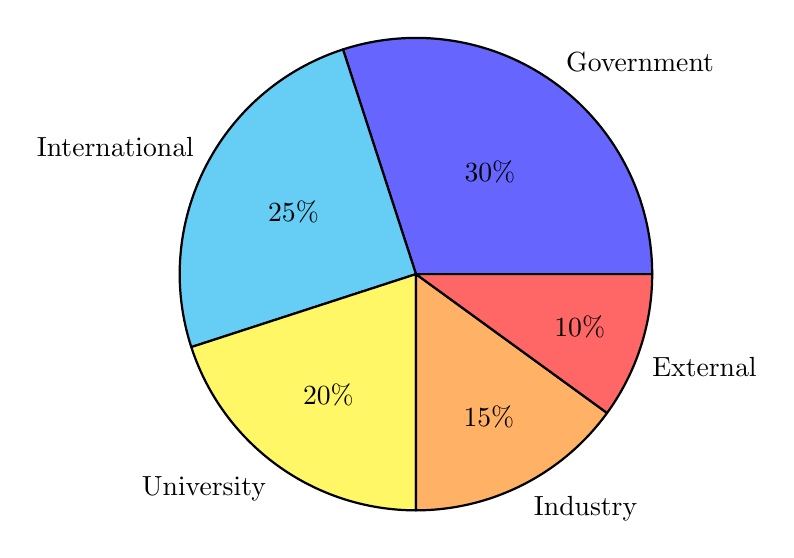
\begin{tikzpicture}
            \pie{30/Government, 25/International, 20/University, 15/Industry, 10/External}
        \end{tikzpicture}
    \end{column}
\end{columns}

\vspace{0.5cm}
\alert{Key Considerations}
\begin{itemize}
    \item Application deadlines vary widely
    \item Each source has specific eligibility criteria
    \item Combine multiple sources when possible
    \item Start your funding search early
\end{itemize}
\end{frame}

% new page
\begin{frame}[fragile]{Financial Aspects of PhD Life}
\begin{columns}[T]
    \begin{column}{0.5\textwidth}
        \alert{Monthly Expenses (Estimated)}
        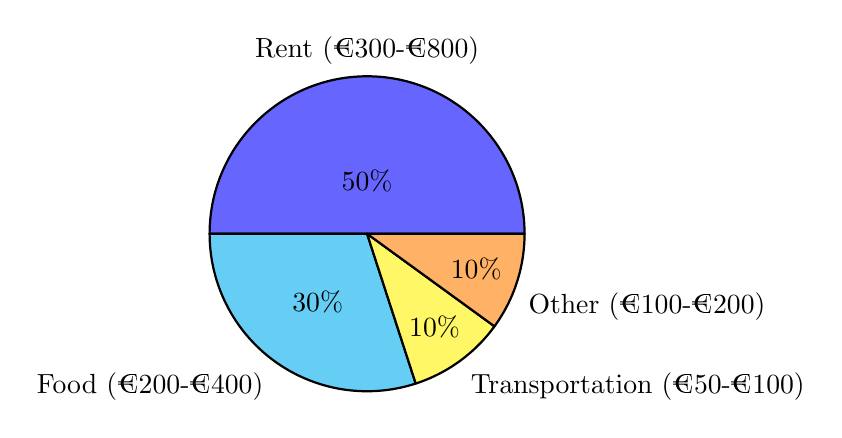
\begin{tikzpicture}
            \pie[radius=2]{
                50/Rent (€300-€800),
                30/Food (€200-€400),
                10/Transportation (€50-€100),
                10/Other (€100-€200)
            }
        \end{tikzpicture}
    \end{column}
    \begin{column}{0.5\textwidth}
        \alert{PhD Salary (TV-L13)}
        \begin{itemize}
            \item 100\% contract: €4200 - €6000 (gross)
            \item 75\% contract: €3150 - €4500 (gross)
            \item Net salary (100\%): €2600 - €3560
        \end{itemize}
        \alert{Benefits}
        \begin{itemize}
            \item Health Insurance
            \item Pension Contributions
            \item 25-30 days Paid Leave
        \end{itemize}
    \end{column}
\end{columns}

\vspace{0.3cm}
\alert{Financial Planning Tips}
\begin{itemize}
    \item Budget for initial setup costs (deposit, furniture)
    \item Consider city-specific cost variations
    \item Explore student discounts and benefits
\end{itemize}
\end{frame}

% new page
\begin{frame}[fragile]{Practical Considerations for PhD Students in Germany}
    \begin{columns}[T]
        \begin{column}{0.33\textwidth}
            \textbf{Work-Life Balance}
            \begin{itemize}
                \item Time management
                \item Goal setting
                \item Progress monitoring
                \item Stress management techniques
            \end{itemize}
        \end{column}
        
        \begin{column}{0.33\textwidth}
            \textbf{Cultural Integration}
            \begin{itemize}
                \item Local events and activities
                \item Student organizations
                \item Language courses
                \item Intercultural workshops
            \end{itemize}
        \end{column}
        
        \begin{column}{0.33\textwidth}
            \textbf{Health and Well-being}
            \begin{itemize}
                \item Health insurance
                \item General practitioner (Hausarzt)
                \item University counseling services
                \item Sports and fitness facilities
            \end{itemize}
        \end{column}
    \end{columns}
    
    \vspace{0.5cm}
    
    \centering\textbf{Remember: Balancing academic pursuits with personal well-being is crucial for PhD success}
\end{frame}


% new page
\begin{frame}[fragile]{Overcoming Challenges in Your PhD Journey}
\begin{columns}[T]
    \begin{column}{0.5\textwidth}
        \alert{Common Challenges}
        \begin{itemize}
            \item Communication with supervisors
            \item Work-life balance
            \item Administrative hurdles
            \item Cultural adaptation
            \item Research setbacks
        \end{itemize}
    \end{column}
    \begin{column}{0.5\textwidth}
        \alert{Effective Solutions}
        \begin{itemize}
            \item Regular supervisor meetings
            \item Clear expectation setting
            \item Utilizing university support services
            \item Peer support networks
            \item Time management techniques
        \end{itemize}
    \end{column}
\end{columns}

\vspace{0.3cm}
\alert{Key Strategies for Success}
\begin{itemize}
    \item Schedule frequent check-ins with supervisors
    \item Seek and provide constructive feedback
    \item Use International Office for visa and integration support
    \item Connect with fellow PhD students for shared experiences
    \item Develop a structured daily routine
\end{itemize}

\begin{tikzpicture}[remember picture,overlay]
%\node[anchor=south east,xshift=-10pt,yshift=10pt] at (current page.south east) {
%    \includegraphics[width=0.2\textwidth]{challenge_icon.png}
%};
\end{tikzpicture}
\end{frame}

% new page
\begin{frame}[fragile]{Building Your Professional Network}
\begin{columns}[T]
    \begin{column}{0.6\textwidth}
        \alert{Networking Opportunities}
        \begin{itemize}
            \item Academic conferences (national \& international)
            \item Professional societies and associations
            \item University workshops and seminars
            \item Online platforms (ResearchGate, Academia.edu)
            \item Industry events and collaborations
        \end{itemize}
    \end{column}
    \begin{column}{0.4\textwidth}
        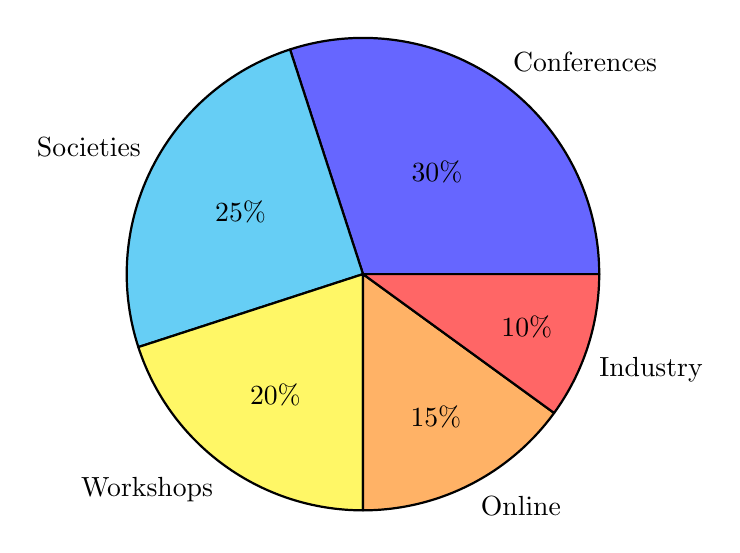
\begin{tikzpicture}
            \pie{30/Conferences, 25/Societies, 20/Workshops, 15/Online, 10/Industry}
        \end{tikzpicture}
    \end{column}
\end{columns}

\vspace{0.3cm}
\alert{Skills to Develop}
\begin{itemize}
    \item Research methodologies
    \item Academic writing and publishing
    \item Presentation and public speaking
    \item Project management
    \item Leadership and team collaboration
\end{itemize}
\end{frame}

% new page
\begin{frame}[fragile]{Maximizing Your Professional Development}
\alert{Effective Networking Strategies}
\begin{itemize}
    \item Be proactive in seeking opportunities
    \item Regularly update your online profiles (LinkedIn, ResearchGate)
    \item Engage in academic discussions (forums, social media)
    \item Volunteer for roles in academic societies
    \item Follow up and maintain professional relationships
\end{itemize}

\vspace{0.3cm}
\alert{Building Your Personal Brand}
\begin{itemize}
    \item Develop a clear research identity
    \item Create and maintain a professional website
    \item Contribute to blogs or write articles in your field
    \item Participate in interdisciplinary collaborations
    \item Seek mentorship opportunities (both as mentee and mentor)
\end{itemize}

\begin{tikzpicture}[remember picture,overlay]
%\node[anchor=south east,xshift=-10pt,yshift=10pt] at (current page.south east) {
%    \includegraphics[width=0.2\textwidth]{network_icon.png}
%};
\end{tikzpicture}
\end{frame}

% new page
\begin{frame}[fragile]{Conclusion: Your PhD Journey Ahead}
\begin{columns}[T]
    \begin{column}{0.6\textwidth}
        \alert{Key Takeaways}
        \begin{itemize}
            \item Diverse funding opportunities
            \item Crucial financial planning
            \item Proactive problem-solving
            \item Continuous networking
            \item Ongoing skill development
        \end{itemize}
        
        \alert{Next Steps}
        \begin{itemize}
            \item Research funding options
            \item Create a personal development plan
            \item Connect with PhD alumni
            \item Explore university resources
        \end{itemize}
    \end{column}
    \begin{column}{0.4\textwidth}
        
\begin{tikzpicture}
            \node[draw, rounded corners, fill=green!20, text width=0.9\textwidth] {
                Your PhD journey in Germany: A challenging but rewarding path to personal and professional growth
            };
        \end{tikzpicture}
    \end{column}
\end{columns}

\vspace{0.5cm}
\centering
\alert{Final Thought}
\Large{Prepare thoroughly, stay resilient, and embrace the opportunities ahead!}
\end{frame}


\end{document}
